\documentclass{article}
\usepackage{amsmath,amsthm}
\usepackage{amssymb}
\usepackage{listings}
\usepackage{flexisym}
\usepackage{graphicx}
%\usepackage{titling}
\makeatletter
\def\tagform@#1{\maketag@@@{[\ignorespaces#1\unskip\@@italiccorr]}}
\makeatother
\title{The Essence of Pushdown Control Flow Analysis \\ and Efficient Application for JavaScript Analysis}
\author{Fei Peng}
\begin{document}
\maketitle
%\tableofcontents
\begin{abstract}
In traditional control flow analysis area, call/return mismatch is always a problem that dramatically reduces precision of analysis. Although, original \textit{k}-CFA uses bounded call strings to acquire limited call/return exact match, this technique causes serious performance cost due to it coupling call/return match strategies with context-sensitivity of values.
Meanwhile, abstracting abstract machine (AAM) a configurable framework for constructing abstract interpreters introduces store-allocated continuation that makes soundness of abstract interpreters easily acquired. Recently, there are three different approaches (PDCFA, AAC, and P4F) published, which provide perfect call/return match for AAM via modeling call stacks as pushdown systems. However, PDCFA needs extra annotated edges to represent stack actions that leads implementing become difficult. AAC requires expensive overhead, and P4F cannot work with monovariance (0-CFA). Consequently, we developed a new method to address the call/return mismatch problem that is extremely easy to implement for ANF style program in abstracting abstract machine. Simultaneously, this method reveals the essence of pushdown control flow analysis, and we exploit the essence to develop a static analyzer for JavaScript with direct abstract syntax tree.

\end{abstract}
\section{Introduction}
\label{Introduction}
Dynamic programming languages (e.g. JavaScript, Python, and Ruby, etc.) play a significant role in a lot of computing areas, such as system management, web development, and scientific computing. Especially, in the past decade, JavaScript becomes a ubiquitous computing environment. However, their certain features (e.g.\ duck-typing, first-class function, highly dynamic object model) make bug detection difficult. Control flow  analysis becomes a good approach to detect deeply semantic defect before actual running programs, but original control flow analysis (\textit{k}-CFA) is too imprecise to apply in realized programs. For example, call/return mismatch is always a problem in \textit{k}-CFA that dramatically reduces precision of analysis.

\lstset{language=Lisp, mathescape}
\begin{lstlisting}

  (let* ((id (lambda (x) x))
         (a (id 1)$^1$)
         (b (id #t)$^2$))
      a)

\end{lstlisting}


Let's consider about the trivial example, in traditional 0-CFA the id function is called twice and \#t finally flows into variable a because there is a spurious flow from call site (id \#t) return to (a (id 1)). In \textit{k}-CFA (k $\geq$ 1), the values of local variable x are distinguished by different call site environments. To illustrate, $(x, 2) \longrightarrow \#t$ means that the value of x is \#t in call site 2, and original \textit{k}-CFA also can use the values' environment to filter inter-procedure control flows, which value of x from call site 2 only can be returned to (b (id \#t)). In this case (non-recursive program), call string with finite length is enough for providing precise call/return flow (value and control flow both). However, any recursive function call will break the rule and propagate spurious information to the whole program. Meanwhile, the performance is unacceptable even when k is 1.

The core idea of pushdown control flow analysis is to mimic call/return flow as a unbounded call stack for ordinary calls, and summarizes the call stack for recursive calls because unbounded call stack is uncomputable in static analysis. CFA2 implements the summarization with a tabulate algorithm, and PDCFA annotates state transition edges with stack actions (push, pop, and no action).Both of CFA2 and PDCFA introduce extra semantics for target languages that makes the abstract interpreters hard to implement.
Fortunately, XXX invented abstracting abstract machine (AAM) as a configurable framework for constructing abstract interpreters in the CESK abstract machine style. AAM not only allocate values in the store (like original \textit{k}-CFA does), but also represents control flow as store-allocated continuations. In AAM, each CESK state does not directly carry continuation, but a continuation address refers to a set of continuations in the store. Merging serval continuations in one continuation address achieves approximation of control flows. Meanwhile, AAM brings two benefits to control flow analysis. On the one hand, it makes soundness of abstract interpreters easily acquired because values and continuations are both in the store and the store size is fixed. On the other hand, store-allocated traditional separates original context-sensitivity (polyvariant values) strategies from call/return match techniques.
AAC and P4F both based on AAM convert call/return match problem to continuation address allocation strategy. AAC requires expensive overhead, $O(n^9)$, which puts too much information in the continuation addresses. Then P4F tries to reduce the complexity of AAC, but it is not useful for monovariant analysis.

In this paper, we introduce a new method to address the call/return mismatch problem that is as simple as P4F and AAC to implement, and it can provide perfect call/return match for monovariant and polyvariant control flow analysis. The new method puts a \emph{execution history environment} into continuation address with callee's function boy, so we name it \textit{h}-CFA\@. The execution history environments can be regarded as call strings with automatically determined length. For non-recursive calls, execution history always provides enough precise context information, no matter how deep the call sequences. On the other hand, execution history can automatically stop growth for recursive calls, and the work list algorithm will be responsible for finding the fixed-point of recursive computation. Furthermore, we claim that for call/return match (polyvariant continuations) finite length of \textit{k} is enough, which can reaches n (size of input program) in worst cases.

We implementeded P4F, PDCFA, PDCFA with GC and \textit{h}-CFA for Scheme, and generated state transition graphs (Figure~\ref{fig:state-graphs}) of these four algorithms for a text program in Figure~\ref{fig:fib}.

\begin{figure}
\small
\begin{center}
\begin{tabular}{ccc}
%\raisebox{1ex-\height}{
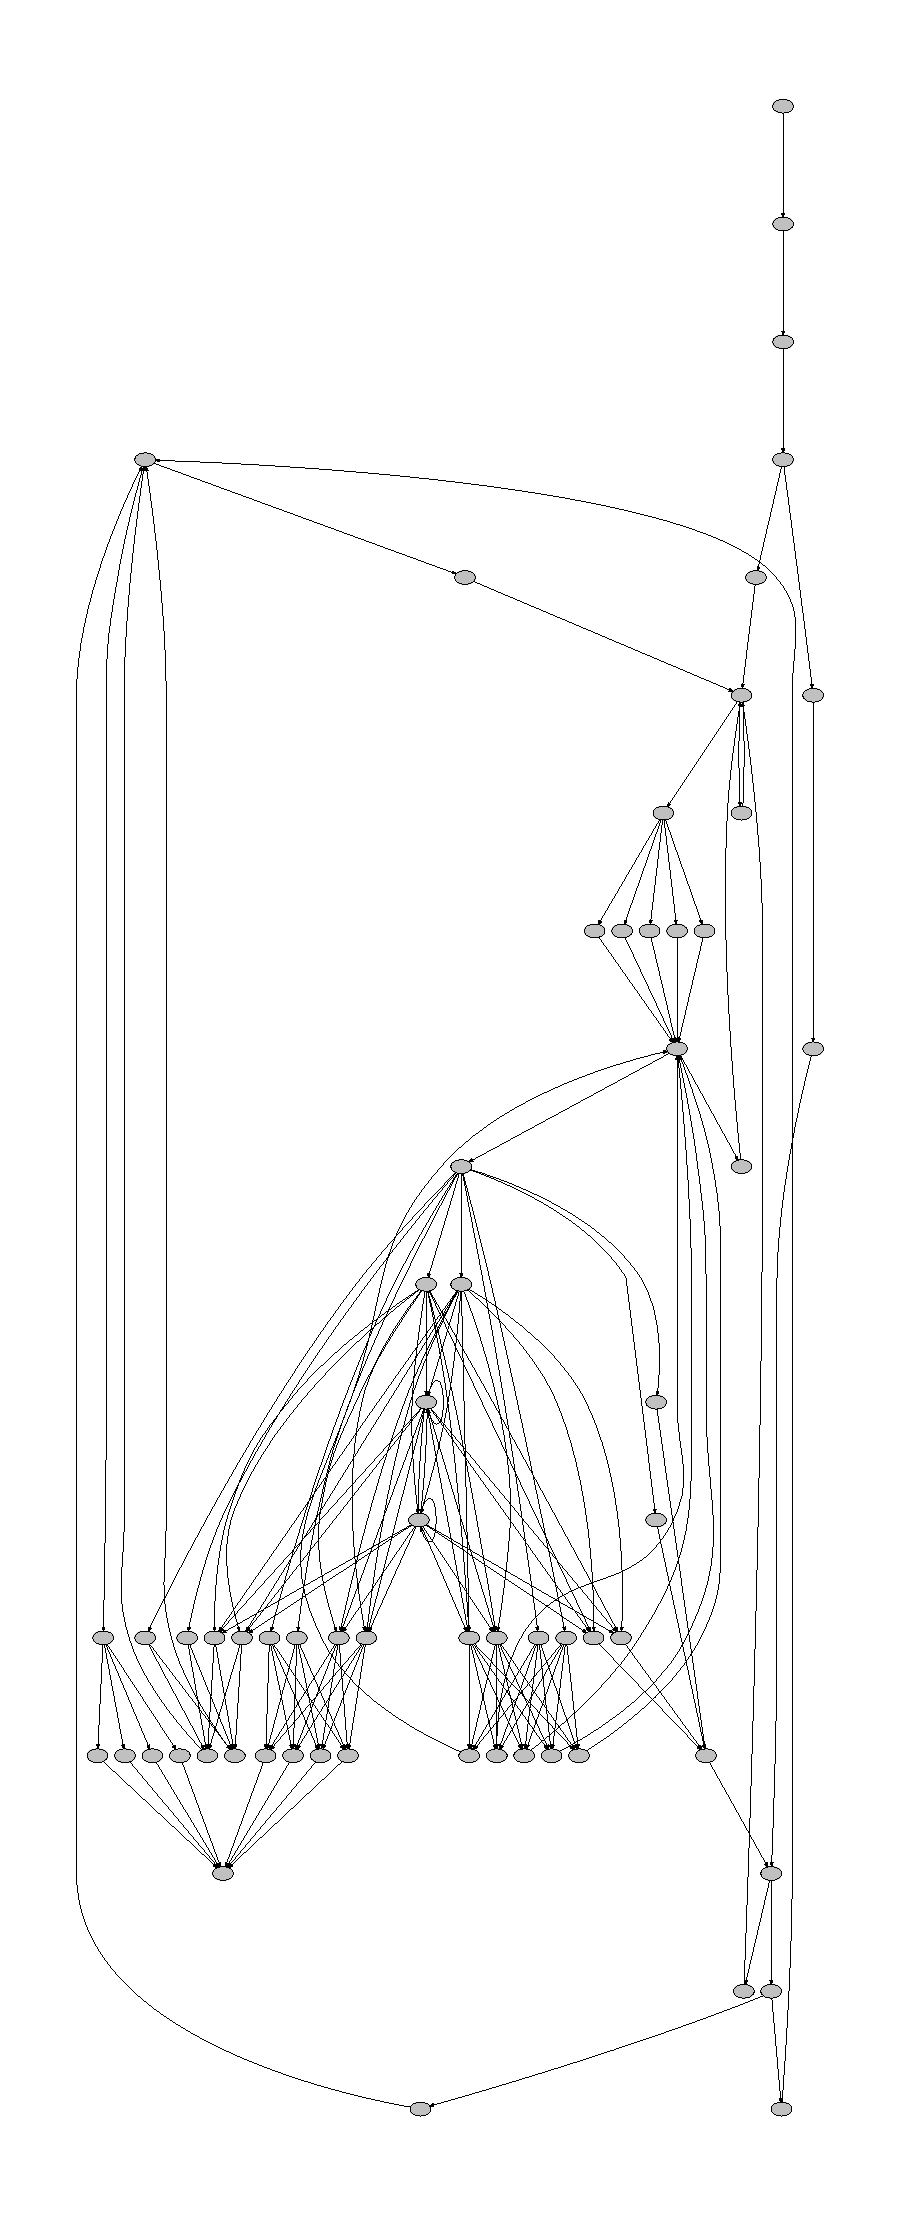
\includegraphics[height=2in]{1p4f.pdf}
%}
&
%\raisebox{1ex-\height}{
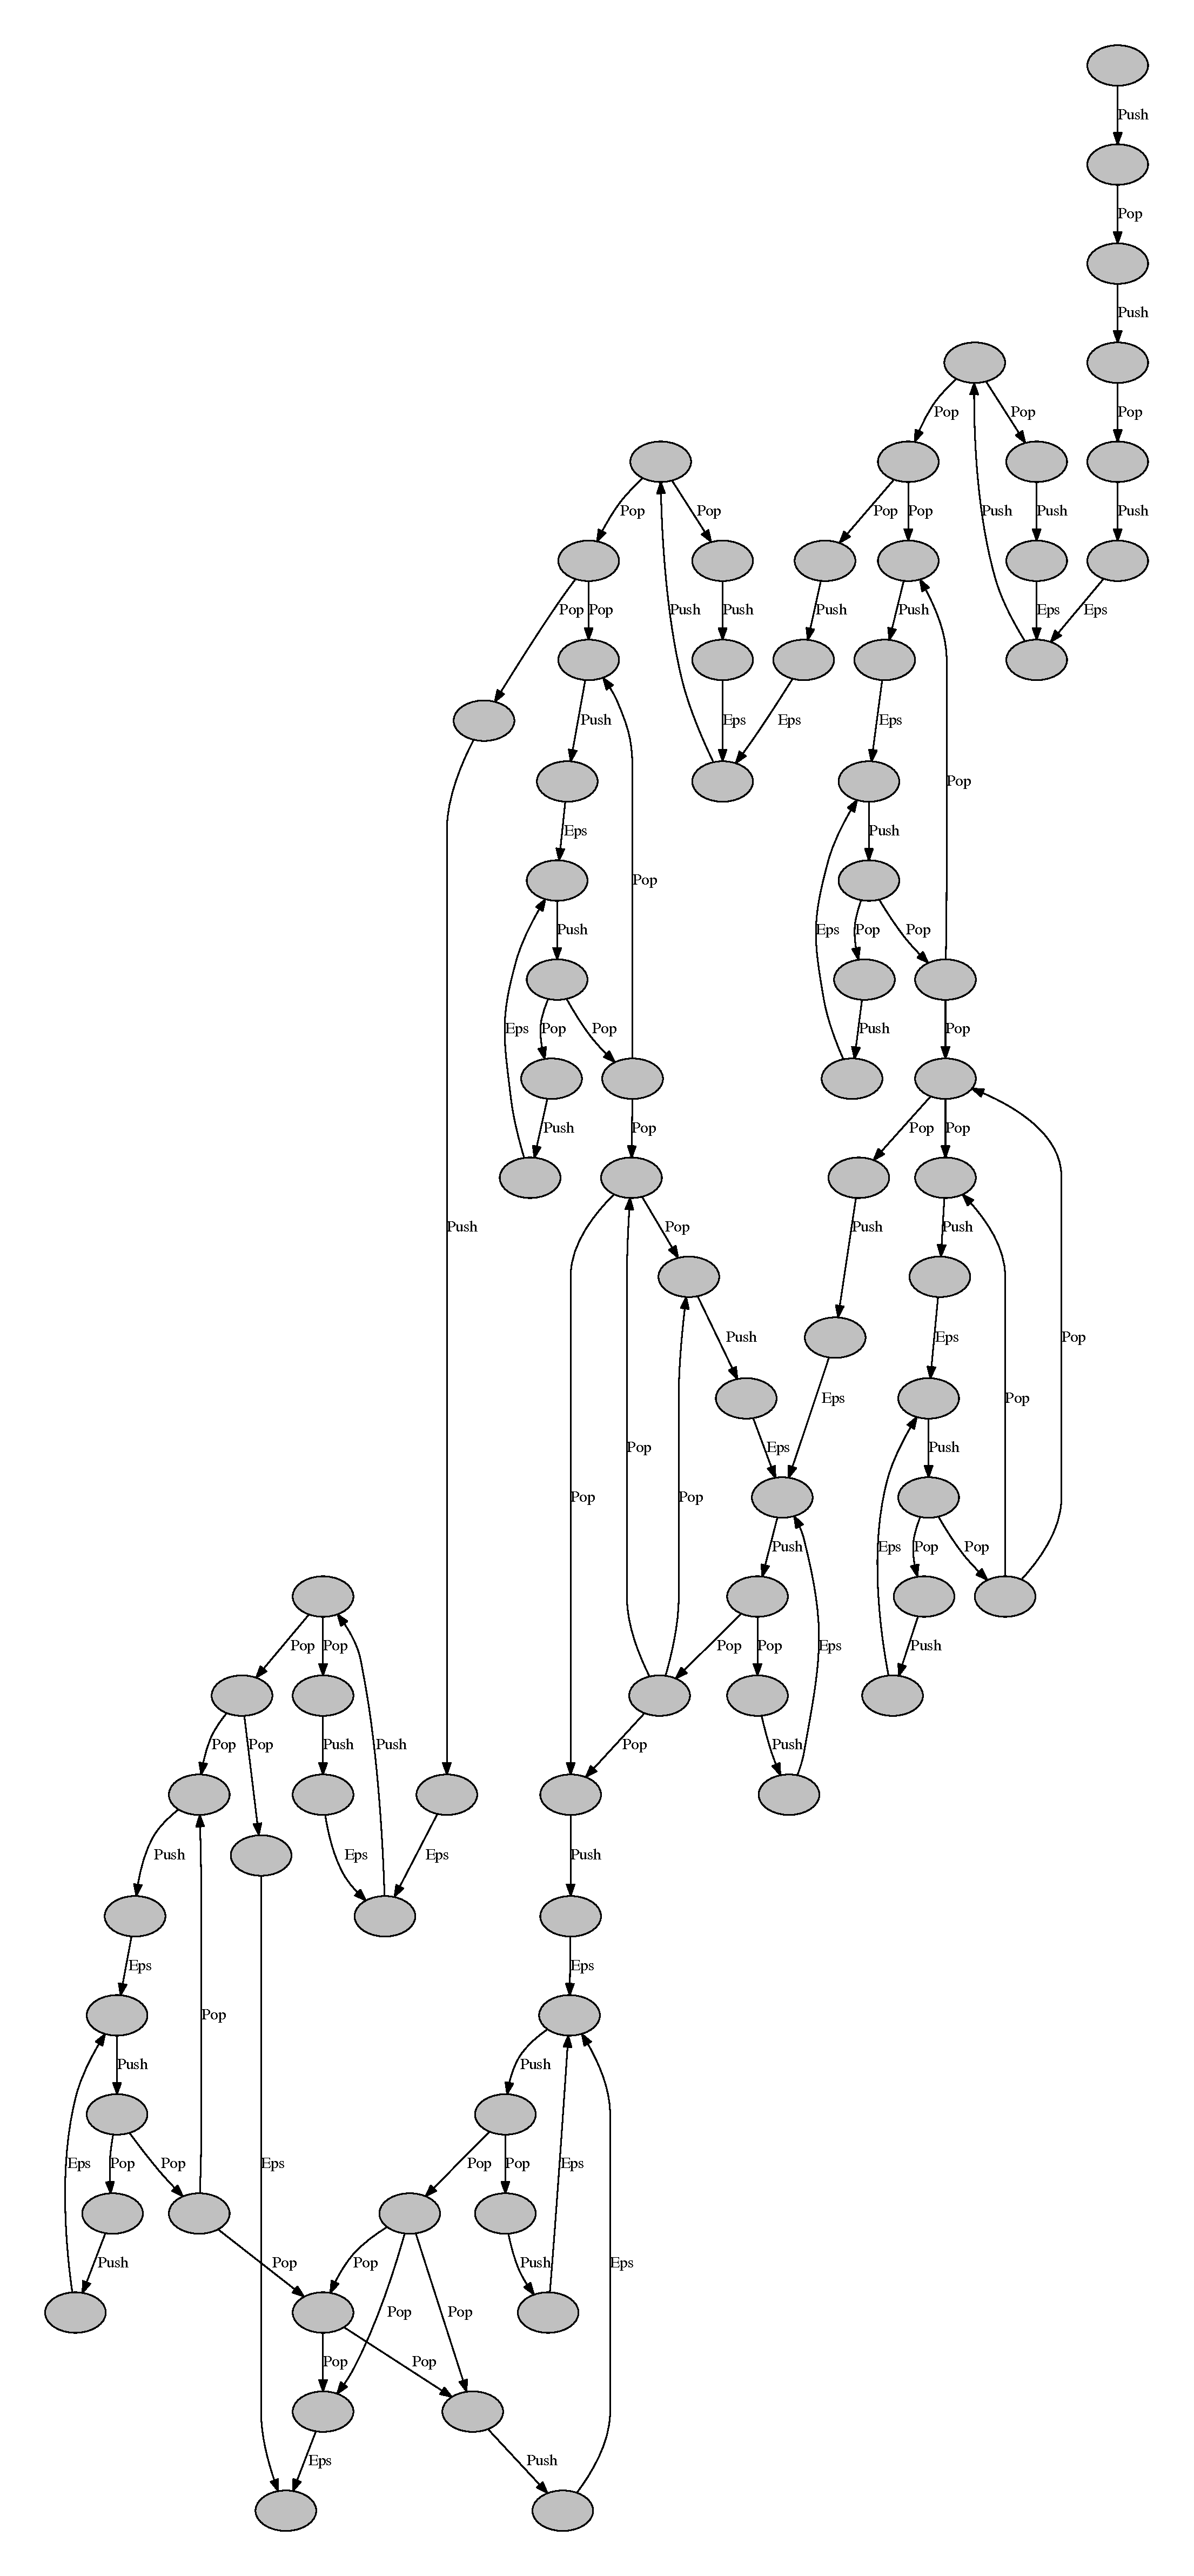
\includegraphics[height=2in]{pdcfaWOgc.pdf}
%}
\\
(a) P4F with 1-call-sensitive
&
(b) PDCFA
\\
%\raisebox{1ex-\height}{
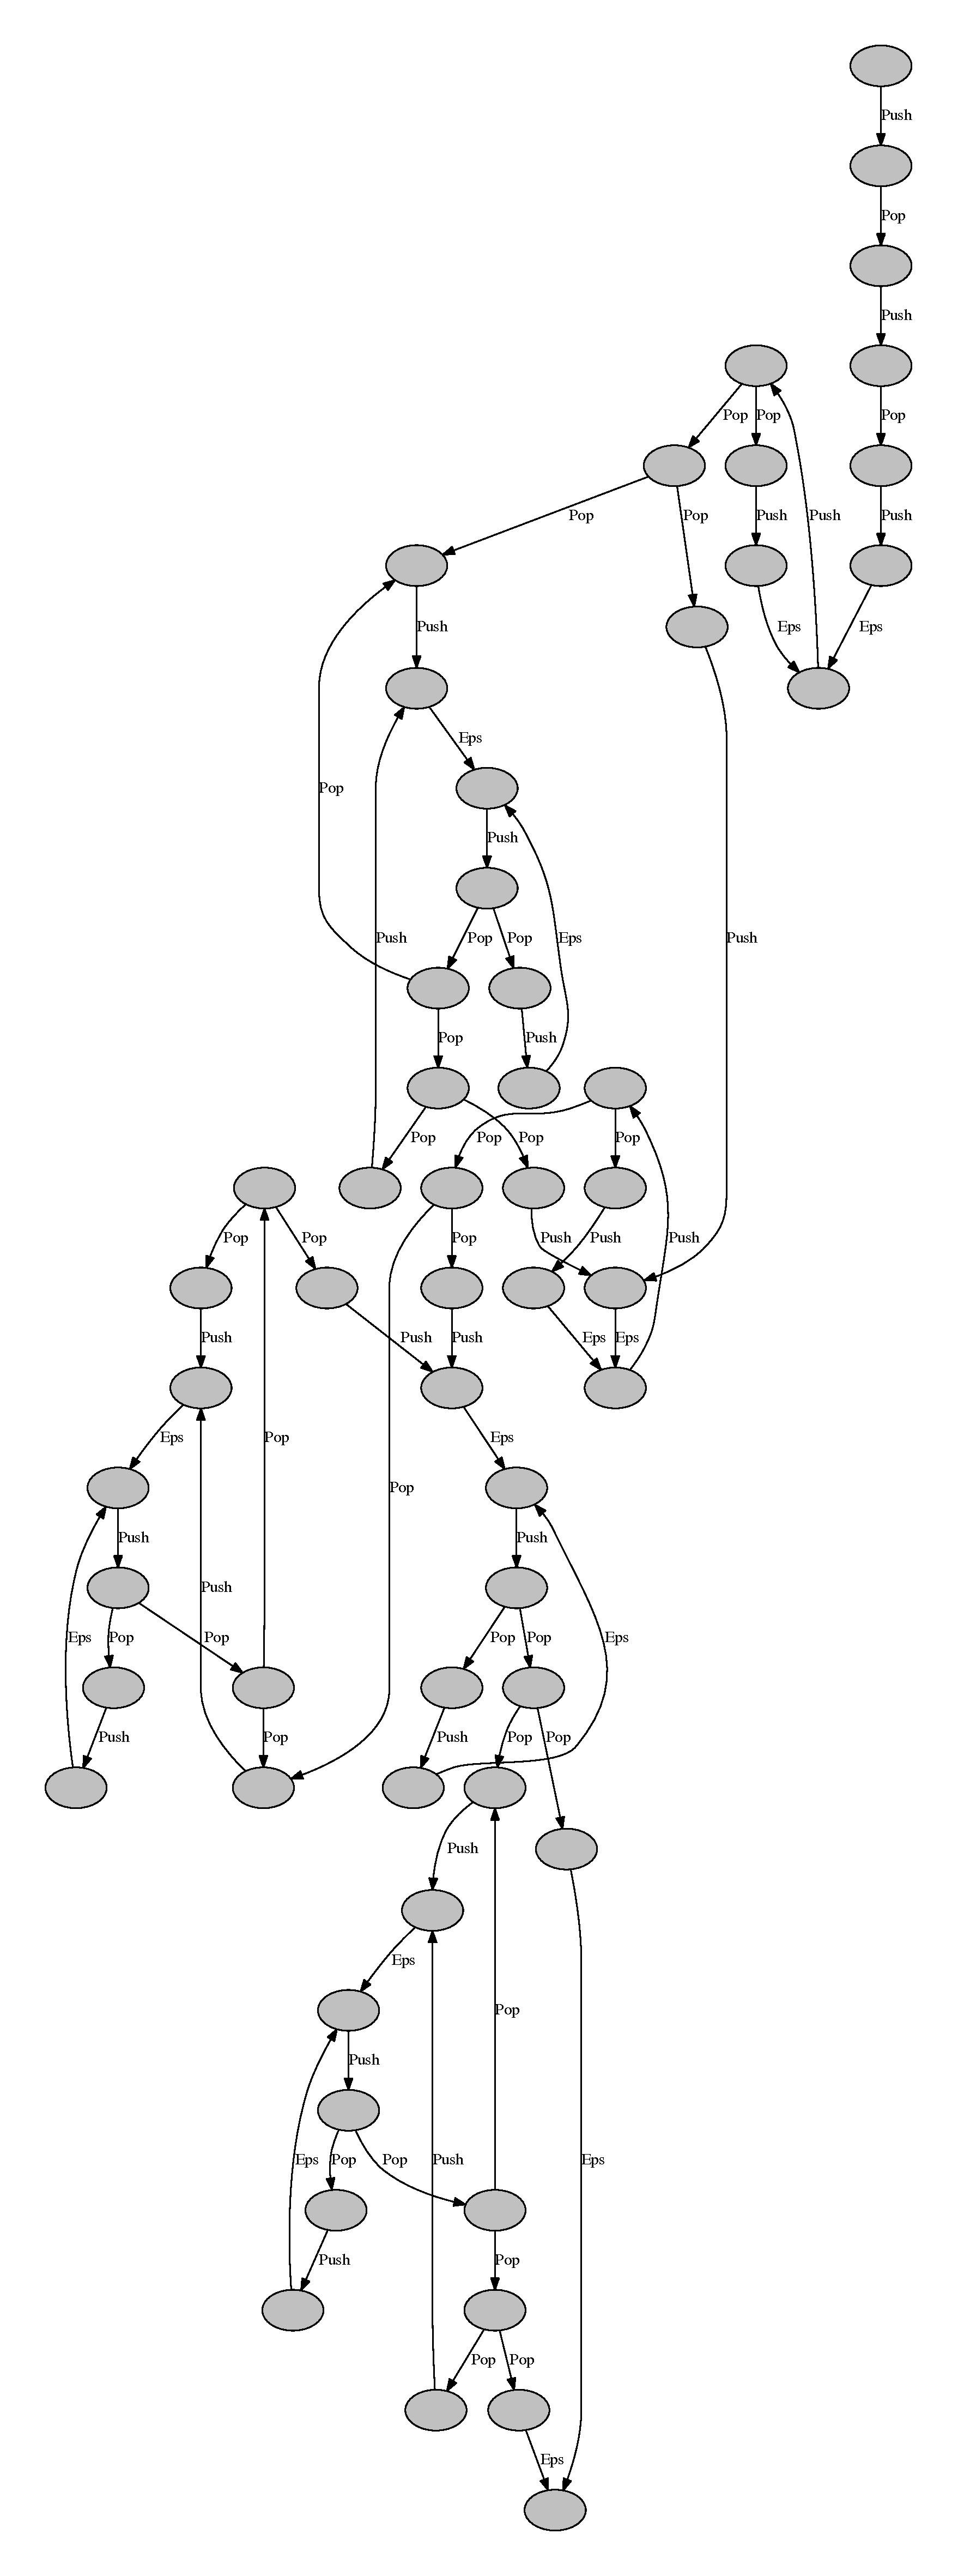
\includegraphics[height=2in]{pdcfa.pdf}
%}
&
%\raisebox{1ex-\height}{
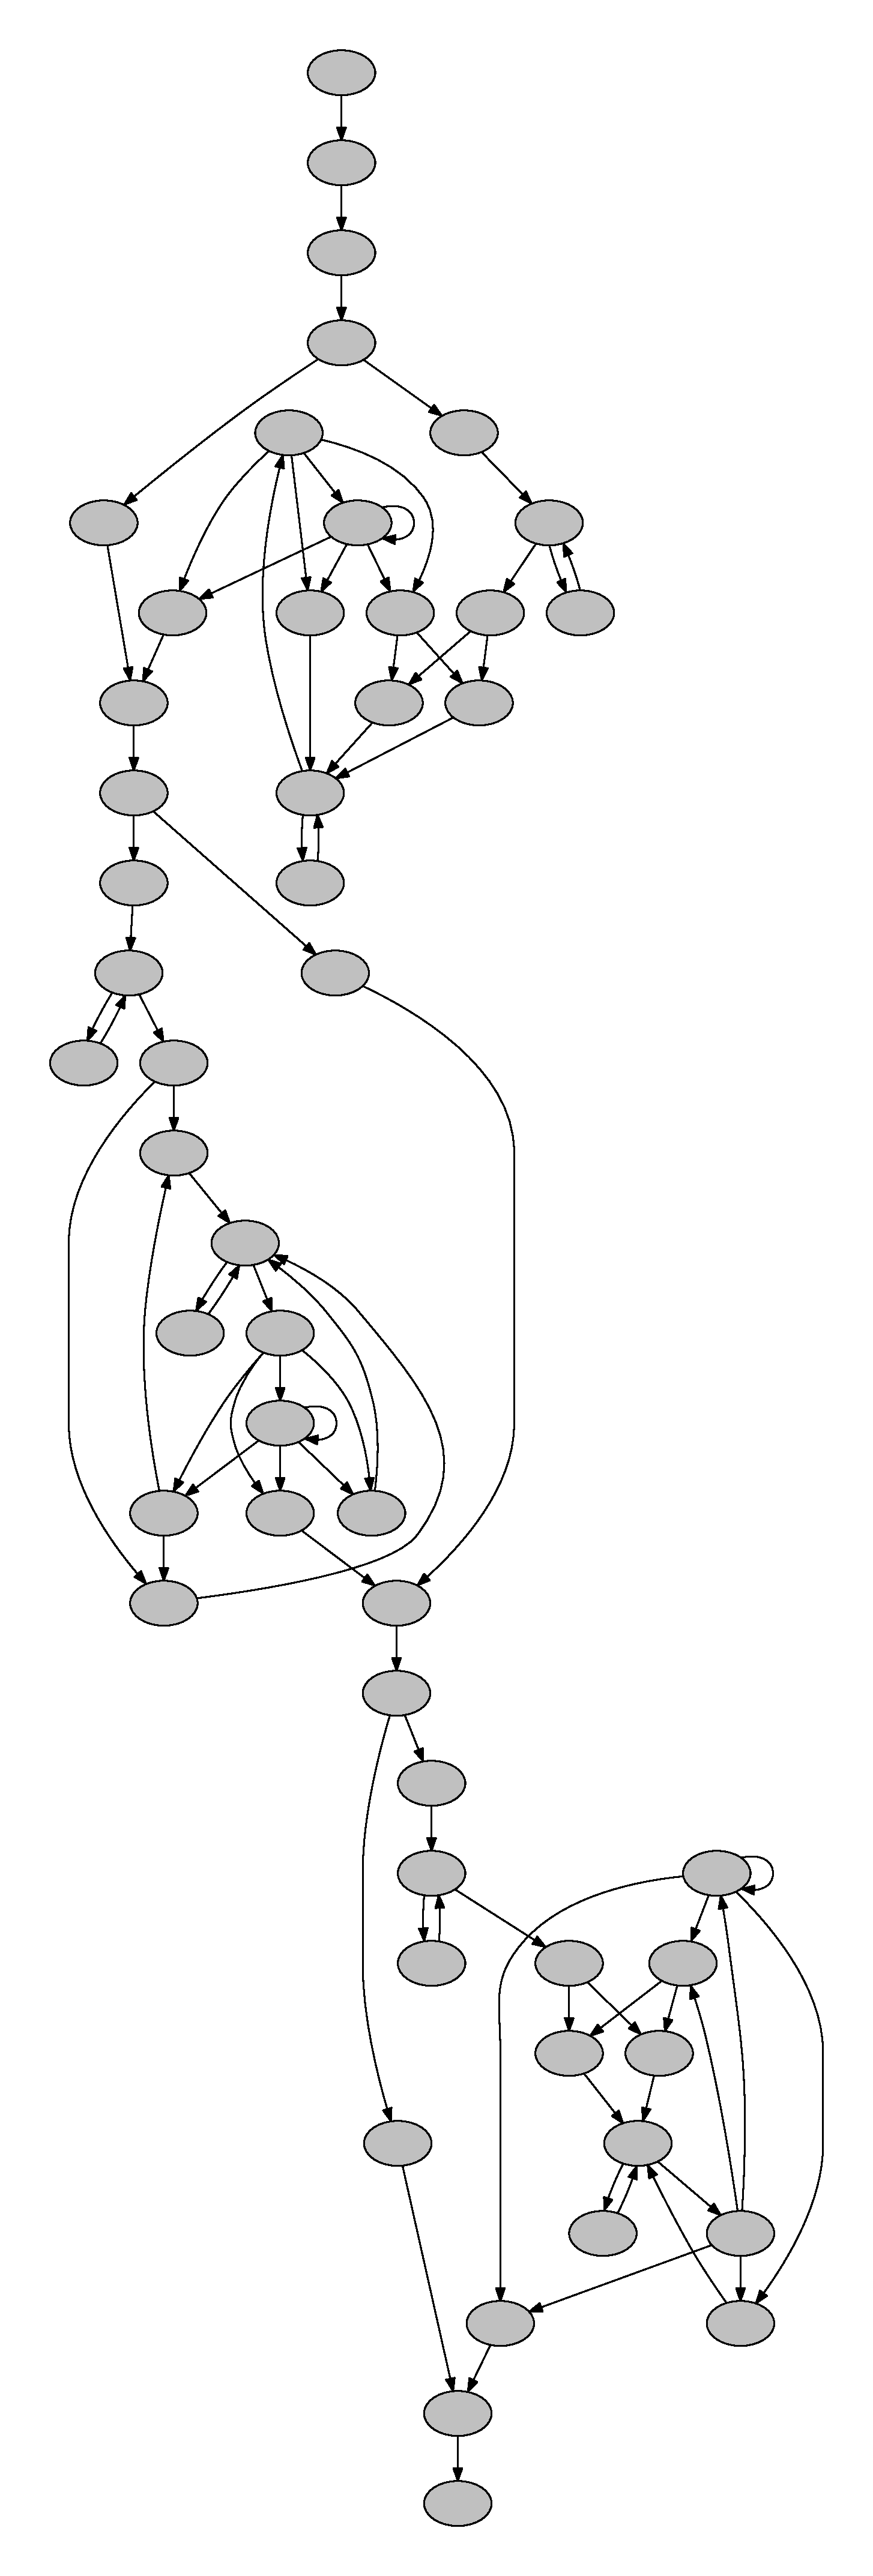
\includegraphics[height=2in]{hcfa.pdf}
%}
\\
(c) PDCFA with Abstract Garbage Collection
&
(d) \textit{h}-CFA
\end{tabular}
\end{center}
\caption{
State transition graphs of: (1) P4F (pushdown control flow analysis for free) with 1-CFA (1-call-site sensitive);
(2) PDCFA (pushdown control flow analysis); (3) PDCFA with abstract garbage collection; (4) \textit{h}-CFA\@.
}
\label{fig:state-graphs}
\end{figure}

\begin{figure}
  \small
  \lstset{language=Lisp}
  \begin{lstlisting}
  (define (fib n)
    (if (< n 3)
        1
        (+ (fib (- n 1)) (fib (- n 2)))))

  (define a (fib 10))
  (define b (fib 20))
  (define c (fib 100))
  \end{lstlisting}
\caption{
The simple example invokes recursive fibonacci function three times on its nontrivial condition.
We use the example to compare call/return match strengths of four pushdown control flow analysis algorithms.
}
\label{fig:fib}
\end{figure}

As the \textit{h}-CFA graph shows, there are three similar subgraphs in the state transition process, which obviously illuminate no call/return flow merged in \textit{h}-CFA due to three subgraphs connected by single transition edges.

\subsection{Overview}
\label{sub:Overview}


\subsection{Contributions}
\label{sub:Contributions}

\section{Pushdown Control Flow Analysis in Abstracting Abstract Machines}
\label{sec:Pushdown Control Flow Analysis in Abstracting Abstract Machines}
\subsection{Abstracting Abstract Machine}
\label{subs:Abstracting Abstract Machine}
Before section 4, we will describe algorithms on ANF style lambda calculus.
\[
\begin{aligned}
\label{eq:bnf}
e \in Exp ::= {}& (let\ ((x\ (f\ ae)))\ e) {} \\
&|\ ae
\end{aligned}
\]
\[
\tag{atomic expressions}
f, ae \in AExp ::= x\ |\ lambda
\]
\[
\tag{lambda abstractions}
lambda \in Lambda ::= (\lambda\ (x)\ e)
\]
\[
\tag{variables}
x,y \in Var \ is\ a\ set\ of\ identifiers
\]

This section reviews AAM\@.

Definitions:

\[
\tag{states}
\widetilde{\varsigma}\in\widetilde{\Sigma} \triangleq Exp \times \widetilde{Env} \times \widetilde{Store}
\times \widetilde{KStore} \times \widetilde{KAddr}
\]
\[
\tag{environments}
\widetilde{\rho} \in \widetilde{Env} \triangleq Var \rightharpoonup \widetilde{Addr}
\]
\[
\tag{srores}
\widetilde{\sigma} \in \widetilde{Store} \triangleq \widetilde{Addr} \mapsto \widetilde{Value}
\]
\[
\tag{abstract values}
\widetilde{v} \in \widetilde{Value} \triangleq \mathcal{P}(\widetilde{Closure})
\]
\[
\tag{closures}
\widetilde{clo} \in \widetilde{Closure} \triangleq Lambda \times \widetilde{Env}
\]
\[
\tag{continuation stores}
\widetilde{\sigma_k} \in \widetilde{KStore} \triangleq  \widetilde{KAddr} \mapsto  \widetilde{Kont}
\]
\[
\tag{abstract continuations}
\widetilde{k} \in  \widetilde{Kont} \triangleq  \mathcal{P}(\widetilde{Frame})
\]
\[
\tag{stack frames}
\widetilde{\phi} \in  \widetilde{Frame} \triangleq Var \times Exp \times  \widetilde{Env} \times  \widetilde{KAddr}
\]
\[
\tag{value addresses}
\widetilde{a} \in \widetilde{Addr} \ is\ a\ finite\ set
\]
\[
\tag{continuation addresses}
\widetilde{a_k} \in \widetilde{KAddr} \ is\ a\ finite\ set
\]

Abstract Semantics:

alloc:
\[
\widetilde{alloc_0} (x, \widetilde{\varsigma}) = x
\]
\[
\widetilde{alloc_1} (x, \widetilde{\varsigma}) = (x, \widetilde{\varsigma})
\]

calls:
\[
\overbrace{
\big((let\ ([y\ (f\ ae)]\ e)), \widetilde{\rho}, \widetilde{\sigma}, \widetilde{\sigma_k}, \widetilde{a_k} \big)
}^{\widetilde{\varsigma}}
\leadsto \big(e\textprime,\widetilde{\rho}\textprime, \widetilde{\sigma}\textprime, \widetilde{\sigma_k}\textprime, \widetilde{a_k}\textprime \big), where
\]
\[
\big((lambda\ (x)\ e\textprime), \widetilde{\rho}_{\lambda}  \big) \in \widetilde{eval}(f, \widetilde{\rho}, \widetilde{\sigma})
\]
\[
\widetilde{\rho}\textprime = \widetilde{\rho}_{\lambda}[x \mapsto \widetilde{a}]
\]
\[
\widetilde{\sigma}\textprime = \widetilde{\sigma} \sqcup [\widetilde{a} \mapsto \widetilde{eval}(ae, \widetilde{\rho}, \widetilde{\sigma})]
\]
\[
\widetilde{a} = \widetilde{alloc}(x, \widetilde{\varsigma})
\]
\[
\widetilde{\sigma_k}\textprime = \widetilde{\sigma_k} \sqcup [\widetilde{a_k}\textprime \mapsto {(y, e, \widetilde{\rho}, \widetilde{a_k})}]
\]
\[
\widetilde{a_k}\textprime = \widetilde{kalloc}(\widetilde{\varsigma}, e\textprime, \widetilde{\rho}\textprime, \widetilde{\sigma}\textprime)
\]


returns:
\[
\overbrace{
(ae, \widetilde{\rho}, \widetilde{\sigma}, \widetilde{\sigma_k}, \widetilde{a_k})
}^{\widetilde{\varsigma}}
\leadsto (e, \widetilde{\rho}\textprime, \widetilde{\sigma}\textprime, \widetilde{\sigma_k}, \widetilde{a_k}\textprime, \widetilde{h}\textprime)
\]
\[
(x, e, \widetilde{\rho_k}, \widetilde{a_k}\textprime) \in \widetilde{\sigma_k}(\widetilde{a_k})
\]
\[
\widetilde{\rho}\textprime = \widetilde{\rho_k}[x \mapsto \widetilde{a}]
\]
\[
\widetilde{\sigma}\textprime = \widetilde{\sigma} \sqcup [\widetilde{a} \mapsto \widetilde{eval}(ae, \widetilde{\rho}, \widetilde{\sigma})]
\]
\[
\widetilde{a} = \widetilde{alloc}(x, \widetilde{\varsigma})
\]

\subsection{Defect of AAM}
\label{sub:Defect of AAM}
Although, abstracting abstract machines import store-allocated values and store-allocated continuations that make call/return match orthogonal from context-sensitivity, original $\widetilde{alloc}$ functions (continuation address allocating strategy) cannot depend upon context information to implement limited call/return match (like \textit{k}-CFA does). P4F attempts to narrow the gap between original \textit{k}-CFA and AAM, so it defines the very simple $\widetilde{alloc}$ function:

\[
\widetilde{kalloc_{P4F}} ((e, \widetilde{\rho}, \widetilde{\sigma}, \widetilde{\sigma_k}, \widetilde{a_k}), e\textprime, \widetilde{\rho}\textprime, \widetilde{\sigma}\textprime) = (e\textprime, \widetilde{\rho}\textprime)
\]

Continuation addresses are represented by $(e\textprime, \widetilde{\rho}\textprime)$ that the most obvious change is it packing callee's function body with ``target environment'' ($\widetilde{\rho}\textprime$) of current application.
Firstly, environments ($Var \rightharpoonup \widetilde{Addr}$) map variable names to value addresses in CESK abstract machines, and AAM encodes polyvatiant strategy (e.g.\ call-site sensitive, object-sensitive, argument-sensitive, etc.) into the value addresses. Thus, P4F can be regarded as an adaptive pushdown control flow analysis algorithm that automatically achieves finite call/return match support from values' polyvatiant strategy (implementing of $\widetilde{alloc}$ function).
Secondly, P4F also reveals a significant fact that why original AAM misses call/return flow match. One of the most important contributions of AAM is that separates analysis context requirement from termination of abstract interpreters. All things (values and continuations) allocated in the store make termination of abstract interpreters easily reached because any implementation of $\widetilde{alloc}$ is sound.
However, the original $\widetilde{kalloc}$ function that mimics generating call stack frames of concrete interpreters does not acquire any benefit from values' polyvariance for getting more precise call/return flow. P4F fixed the problem by introducing polyvariance into continuation store, which brings context information in target environment to distinguish continuations under different contexts. Although P4F cannot perfect match call/return flow infinitely, it still discovers the essence of pushdown control flow analysis in AAM\@: continuations also need to be polyvariant (context-sensitive) to achieve more precise static analysis result.

\section{The Essence of Pushdown Control Flow Analysis}
\label{sec:The Essence of Pushdown Control Flow Analysis}
Inspired by P4F, we deem that pushdown analysis (polyvariant continuation store) is orthogonal from polyvariant store, in other words, control flow analysis can get call/return match that does not depend on polyvariant store. Simultaneously, we try to find the proper contexts for polyvariant continuations.

This section describes $CESK^H$ machines that record ``program execution history'' into each abstract machine state.
The program execution history records and summarizes execution path from the beginning of program to current state.
During evaluating function calls, the program execution history uniquely represents current call site in continuation store.


\subsection{Program Execution History}
\label{sub:Program Execution History}
First, we modify the $CESK$ machine defined in Section~\ref{subs:Abstracting Abstract Machine} to $CESK^H$ machine.
Data types and notations of $CESK^H$ are defined below.

\[
\tag{states}
\widetilde{\varsigma^H}\in\widetilde{\Sigma^H} \triangleq Exp \times \widetilde{Env} \times \widetilde{Store}
\times \widetilde{KStore^H} \times \widetilde{KAddr^H} \times \widetilde{History}
\]
\[
\tag{environments}
\widetilde{\rho} \in \widetilde{Env} \triangleq Var \rightharpoonup \widetilde{Addr}
\]
\[
\tag{srores}
\widetilde{\sigma} \in \widetilde{Store} \triangleq \widetilde{Addr} \mapsto \widetilde{Value}
\]
\[
\tag{abstract values}
\widetilde{v} \in \widetilde{Value} \triangleq \mathcal{P}(\widetilde{Closure})
\]
\[
\tag{closures}
\widetilde{clo} \in \widetilde{Closure} \triangleq Lambda \times \widetilde{Env}
\]
\[
\tag{continuation stores}
\widetilde{\sigma_k^H} \in \widetilde{KStore^H} \triangleq  \widetilde{KAddr^H} \mapsto  \widetilde{Kont^H}
\]
\[
\tag{abstract continuations}
\widetilde{k^H} \in  \widetilde{Kont^H} \triangleq  \mathcal{P}(\widetilde{Frame^H})
\]
\[
\tag{stack frames}
\widetilde{\phi^H} \in  \widetilde{Frame^H} \triangleq Var \times Exp \times  \widetilde{Env} \times \widetilde{History} \times  \widetilde{KAddr^H}
\]
\[
\tag{histories}
\widetilde{h} \in \widetilde{History} \triangleq Var \rightharpoonup \widetilde{Addr}
\]
\[
\tag{value addresses}
\widetilde{a} \in \widetilde{Addr} \ is\ a\ finite\ set
\]
\[
\tag{continuation addresses}
\widetilde{a_k^H} \in \widetilde{KAddr} \ is\ a\ finite\ set
\]

In ANF programs, environment naturally maintains intro-procedural execution history because ANF explicitly extracts intro-procedural control flows in let-bindings and saves every intermediate result in a local variable.
Consequently, the program execution histories can be implemented as propagating environments by $\widetilde{History}$ field of $CESK^H$ machine states.
The execution history can be regarded as call strings with automatically determined length. For non-recursive calls, execution history always provides enough precise context information, no matter how deep the call sequences. On the other hand, execution history can automatically stop growth for recursive calls, and the work list algorithm will be responsible for finding the fixed-point of recursive computation.

Following definitions describe the abstract semantics of $CESK^H$ machine.

Calls:
\[
\overbrace{
\big((let\ ([y\ (f\ ae)]\ e)), \tilde{\rho}, \tilde{\sigma}, \tilde{\sigma_k}, \tilde{a_k}, \tilde{h} \big)
}^{\widetilde{\varsigma^H}}
\leadsto \big(e\textprime,\tilde{\rho}\textprime, \tilde{\sigma}\textprime, \widetilde{\sigma_k^H}\textprime, \widetilde{a_k^H}\textprime, \tilde{h}\textprime \big), where
\]
\[
\big((lambda\ (x)\ e\textprime), \tilde{\rho}_{\lambda}  \big) \in \widetilde{eval}(f, \tilde{\rho}, \tilde{\sigma})
\]
\[
\tilde{\rho}\textprime = \tilde{\rho}_{\lambda}[x \mapsto \tilde{a}]
\]
\[
\tilde{\sigma}\textprime = \tilde{\sigma} \sqcup [\tilde{a} \mapsto \widetilde{eval}(ae, \tilde{\rho}, \tilde{\sigma})]
\]
\[
\tilde{a} = \widetilde{alloc}(x, \widetilde{\varsigma^H})
\]
\[
\widetilde{\sigma_k^H}\textprime = \widetilde{\sigma_k^H} \sqcup [\widetilde{a_k^H}\textprime \mapsto {(y, e, \tilde{\rho}, \tilde{h}, \widetilde{a_k^H})}]
\]
\[
\widetilde{a_k^H}\textprime = \widetilde{kalloc_h}(\tilde{\varsigma}, e\textprime, \tilde{\rho}\textprime, \tilde{\sigma}\textprime)
\]
\[
\tilde{h}\textprime = \tilde{h}[x \mapsto \tilde{a}]
\]

Returns:
\[
\overbrace{
(ae, \tilde{\rho}, \tilde{\sigma}, \tilde{\sigma_k}, \widetilde{a_k^H}, \tilde{h})
}^{\widetilde{\varsigma^H}}
\leadsto (e, \tilde{\rho}\textprime, \tilde{\sigma}\textprime, \widetilde{\sigma_k^H}, \widetilde{a_k^H}\textprime, \tilde{h}\textprime)
\]
\[
(x, e, \tilde{\rho_k}, \tilde{h_k}, \widetilde{a_k^H}\textprime) \in \widetilde{\sigma_k^H}(\widetilde{a_k^H})
\]
\[
\tilde{\rho}\textprime = \tilde{\rho_k}[x \mapsto \tilde{a}]
\]
\[
\tilde{\sigma}\textprime = \tilde{\sigma} \sqcup [\tilde{a} \mapsto \widetilde{eval}(ae, \tilde{\rho}, \tilde{\sigma})]
\]
\[
\tilde{a} = \widetilde{alloc}(x, \widetilde{\varsigma^H})
\]
\[
\tilde{h}\textprime = \tilde{h_k}[x \mapsto \tilde{a}]
\]

Above definitions propagate execution history by adding current . Then $\widetilde{kalloc_h}$ function takes the execution history to compute the unique continuation address for corresponding call site.
\[
\widetilde{kalloc_h} ((e, \widetilde{\rho}, \widetilde{\sigma}, \widetilde{\sigma_k^H}, \widetilde{a_k^H}, \widetilde{h}), e\textprime, \widetilde{\rho}\textprime, \widetilde{\sigma}\textprime) =
(e, e\textprime, \widetilde{h})
\]

\subsection{Polyvariant Continuation}
\label{sub:Polyvariant Continuation}
Let's exam the analysis process of a simple example to understand \textit{h}-CFA, the example is similar with Figure~\ref{fig:fib} but written in ANF style showed by Figure~\ref{fig:anf-fib}.

\begin{figure}[h]
\small
\lstset{language=Lisp}
\begin{lstlisting}
  (letrec ((fib (lambda (n)
                  (let ((res1 (< n 3)))
                    (if res1
                        1
                        (let* ((res2 ($-$ n 1))
                               (res3 (fib res2))
                               (res4 ($-$ n 2))
                               (res5 (fib res4))
                               (res6 (+ res3 res5)))
                            res6))))))
    (let ((a (fib 10))
          (b (fib 20)))
      $\dots$))
\end{lstlisting}
\caption{
We rewrite the former example in ANF style.
For convenient  demonstrating, we use complete Scheme language with numbers and booleans instead of pure lambda calculus.
}
\label{fig:anf-fib}
\end{figure}

In this subsection, execution histories are briefly represented as variable sequences, and callee's function body (the first part of $\widetilde{KAddr^H}$) is replaced by the function name. This temporary convince just makes the explanation more readable but not actually modify the abstract semantics of $CESK^H$ machines.

Through steps of the abstract interpreter, the first call site (a (fib 10)) carries history $\{fib\}$ that means in this program point we only finished computing the declaration of function ``fib''.
Thus, the continuation (call stack frame) of the call site is allocated at $(fib, \{fib\})$, and the stack frame looks like $(a, (let\ (b\ (fib\ 20))\ \dots), \widetilde{env_1}, \{fib\}, \widetilde{a_k{}_{init}})$ that is the one and only element of the continuation store so far.
The stack frame expresses that after complete this invocation,
(1) return value will be stored in variable ``a'',
(2) the computation will shift to $(let\ (b\ (fib\ 20))\ \dots)$ with environment $\widetilde{env_1}$,
(3) and recover continuation address $\widetilde{a_k{}_{init}}$ a fake continuation address representing top level's continuation.

After diving into the callee's function body, the second call appears at (res3 (fib res2)). At this point, the execution history $\{fib, res1, res2\}$ is different from the history of last call site, so the continuation store contains two abstract continuations with distinct addresses.
\[
\widetilde{a^H_k{}_1} = ((fib\ 10), fib, \{fib\})
\]
\[
\widetilde{a^H_k{}_2} = ((fib\ res2), fib, \{fib, res1, res2\})
\]
\[
\begin{aligned}
\label{eq:show-stack}
\widetilde{\sigma_k^H} = \{ {}& \widetilde{a^H_k{}_1} \mapsto \{(a, (let\ (b\ (fib\ 20))\ \dots), \widetilde{env_1}, \{fib\}, \widetilde{a^H_k{}_{init}})\}  {} \\
                              & \widetilde{a^H_k{}_2} \mapsto \{(res3, (let\ (res4\ (-\ n\ 2)) \dots), \widetilde{env_2}, \{fib, res1, res2\}, \tilde{a^H_k{}_1})\} \}
\end{aligned}
\]

As above illustration shows, the continuation store is a linked stack structure. Each frame has a $\widetilde{a^H_k}$ that points to the next frame in the stack. This stack-like structure perfect mimics call stacks of concrete interpreters. Certainly, the call stie (fib res4) will also gets its own execution history after computation of (fib res2) becomes complete (acquired its fixed-point).

\[
\widetilde{a^H_k{}_3} = ((fib\ res4), fib, \{fib, res1, res2, res3, res4\})
\]

However, (res3 (fib res2)) is a recursive call site, so the execution history at this point will not be added new element to distinguish (res3 (fib res2)) from its variances of different recursive levels. Thus, control flows from multiple recursive levels of a call site are merged into one continuation address. Eventually, there are three frames merged into $\widetilde{a^H_k{}_2}$, but this merge does not lead ``static'' call/return mismatch. All of the frames merged into $\widetilde{a^H_k{}_2}$ can bring control flow back to set ``res3''.

\[
\begin{aligned}
\label{eq:show-stack}
\widetilde{a^H_k{}_2} \mapsto \{ {}& (res3, (let\ (res4\ (-\ n\ 2)) \dots), \widetilde{env_2}, \tilde{h_2}, \widetilde{a^H_k{}_1}), {} \\
                                 {}& (res3, (let\ (res4\ (-\ n\ 2)) \dots), \widetilde{env_a}, \tilde{h_a}, \widetilde{a^H_k{}_2}) \}
\end{aligned}
\]

The merging expresses a fact that the invocation of ``fib'' at point (fib res2) may be made by (a (fib 10)) or (res3 (fib res2)). Moreover, the second frame in above illustration has the ``next'' pointer $\widetilde{a^H_k{}_2}$ that refers to itself. This cycle makes the continuation store no longer stack-like, but a graph.

After compute (a (fib 10), the function ``fib'' is called again by (b (fib 20)). At this point, $\widetilde{kalloc_h}$ generates a new continuation address.

\[
\widetilde{a^H_k{}_4} = ((fib\ 20), fib, \{fib, a\})
\]

The execution history of this point becomes $\{fib, a\}$ that summarize the execution path of computing (a (fib 10)) to ``a''. In other words, the program execution history just cares about which portions of the program we have done, but it ignores how we got them. This summarization limits length of execution histories under \textit{n} (the size of input program) in worst cases.

Then the abstract interpreter restarts to execute the function and encounters call site (res3 (fib res2)) again. At this time, the continuation address allocated for call site (res3 (fib res2)) differs from last time.

\[
\widetilde{a^H_k{}_5} = ((fib\ res2), fib, \{fib, a, res1, res2\})
\]

\subsection{Store-widenning}
\label{sub:Store-widenning}

\subsection{Defect of \textit{h}-CFA}
\label{sub:Defect of h-CFA}


\section{Static Analysis of JavaScript}
\label{sec:Static Analysis of JavaScript}
\subsection{Abstract Garbage Collection as Stack Filtering}
\label{sub:Abstract Garbage Collection as Stack Filtering}
In practice, call/return perfect match working with monovariant analysis is useless.
\subsection{Abstract Garbage Collection as Popping Call Stack Frames}
\label{sub:Abstract Garbage Collection as Popping Call Stack Frames}
In this section, we show how to give up execution history and apply our theory for direct-style AST\@.
\end{document}
